
\section{Experiments}
We evaluate REPMD and PMAC on a number of benchmark tasks. We first introduce the experimented tasks, then present the experiment results. Implementation details are provided in \cref{subsec:implementation}. 

\subsection{Tasks}
\label{subsec:tasks}
We test the performance of REPMD on a synthetic bandit problem and the algorithmic tasks from OpenAI gym library \citep{brockman2016openai}. The synthetic multi-armed bandit problem has 10,000 distinct actions. The reward of each action $i$ is initialized by $r_i = s_i^{8}$, where $s_i$ is randomly sampled from a uniform distribution over $[0,1)$. Each action $i$ is represented by a randomly sampled feature vector $\phi_i\in \mathbb{R}^{20}$ from standard normal distribution. Note that these features are fixed during training. We further test our method on five algorithmic tasks from the OpenAI gym library, in rough order of difficulty: Copy, DuplicatedInput, RepeatCopy, Reverse, and ReversedAddition \citep{brockman2016openai}. Lastly, we test PMAC using standard continuous-control benchmarks from OpenAI Gym utilizing the Mujoco environment \citep{brockman2016openai,todorov2012mujoco}, including Hopper, Walker2d, HalfCheetah, Ant and Humanoid. The details of algorithmic and mujoco tasks are provided in \cref{subsec:benchmarks}. 

\begin{figure*}[t]
\begin{center}
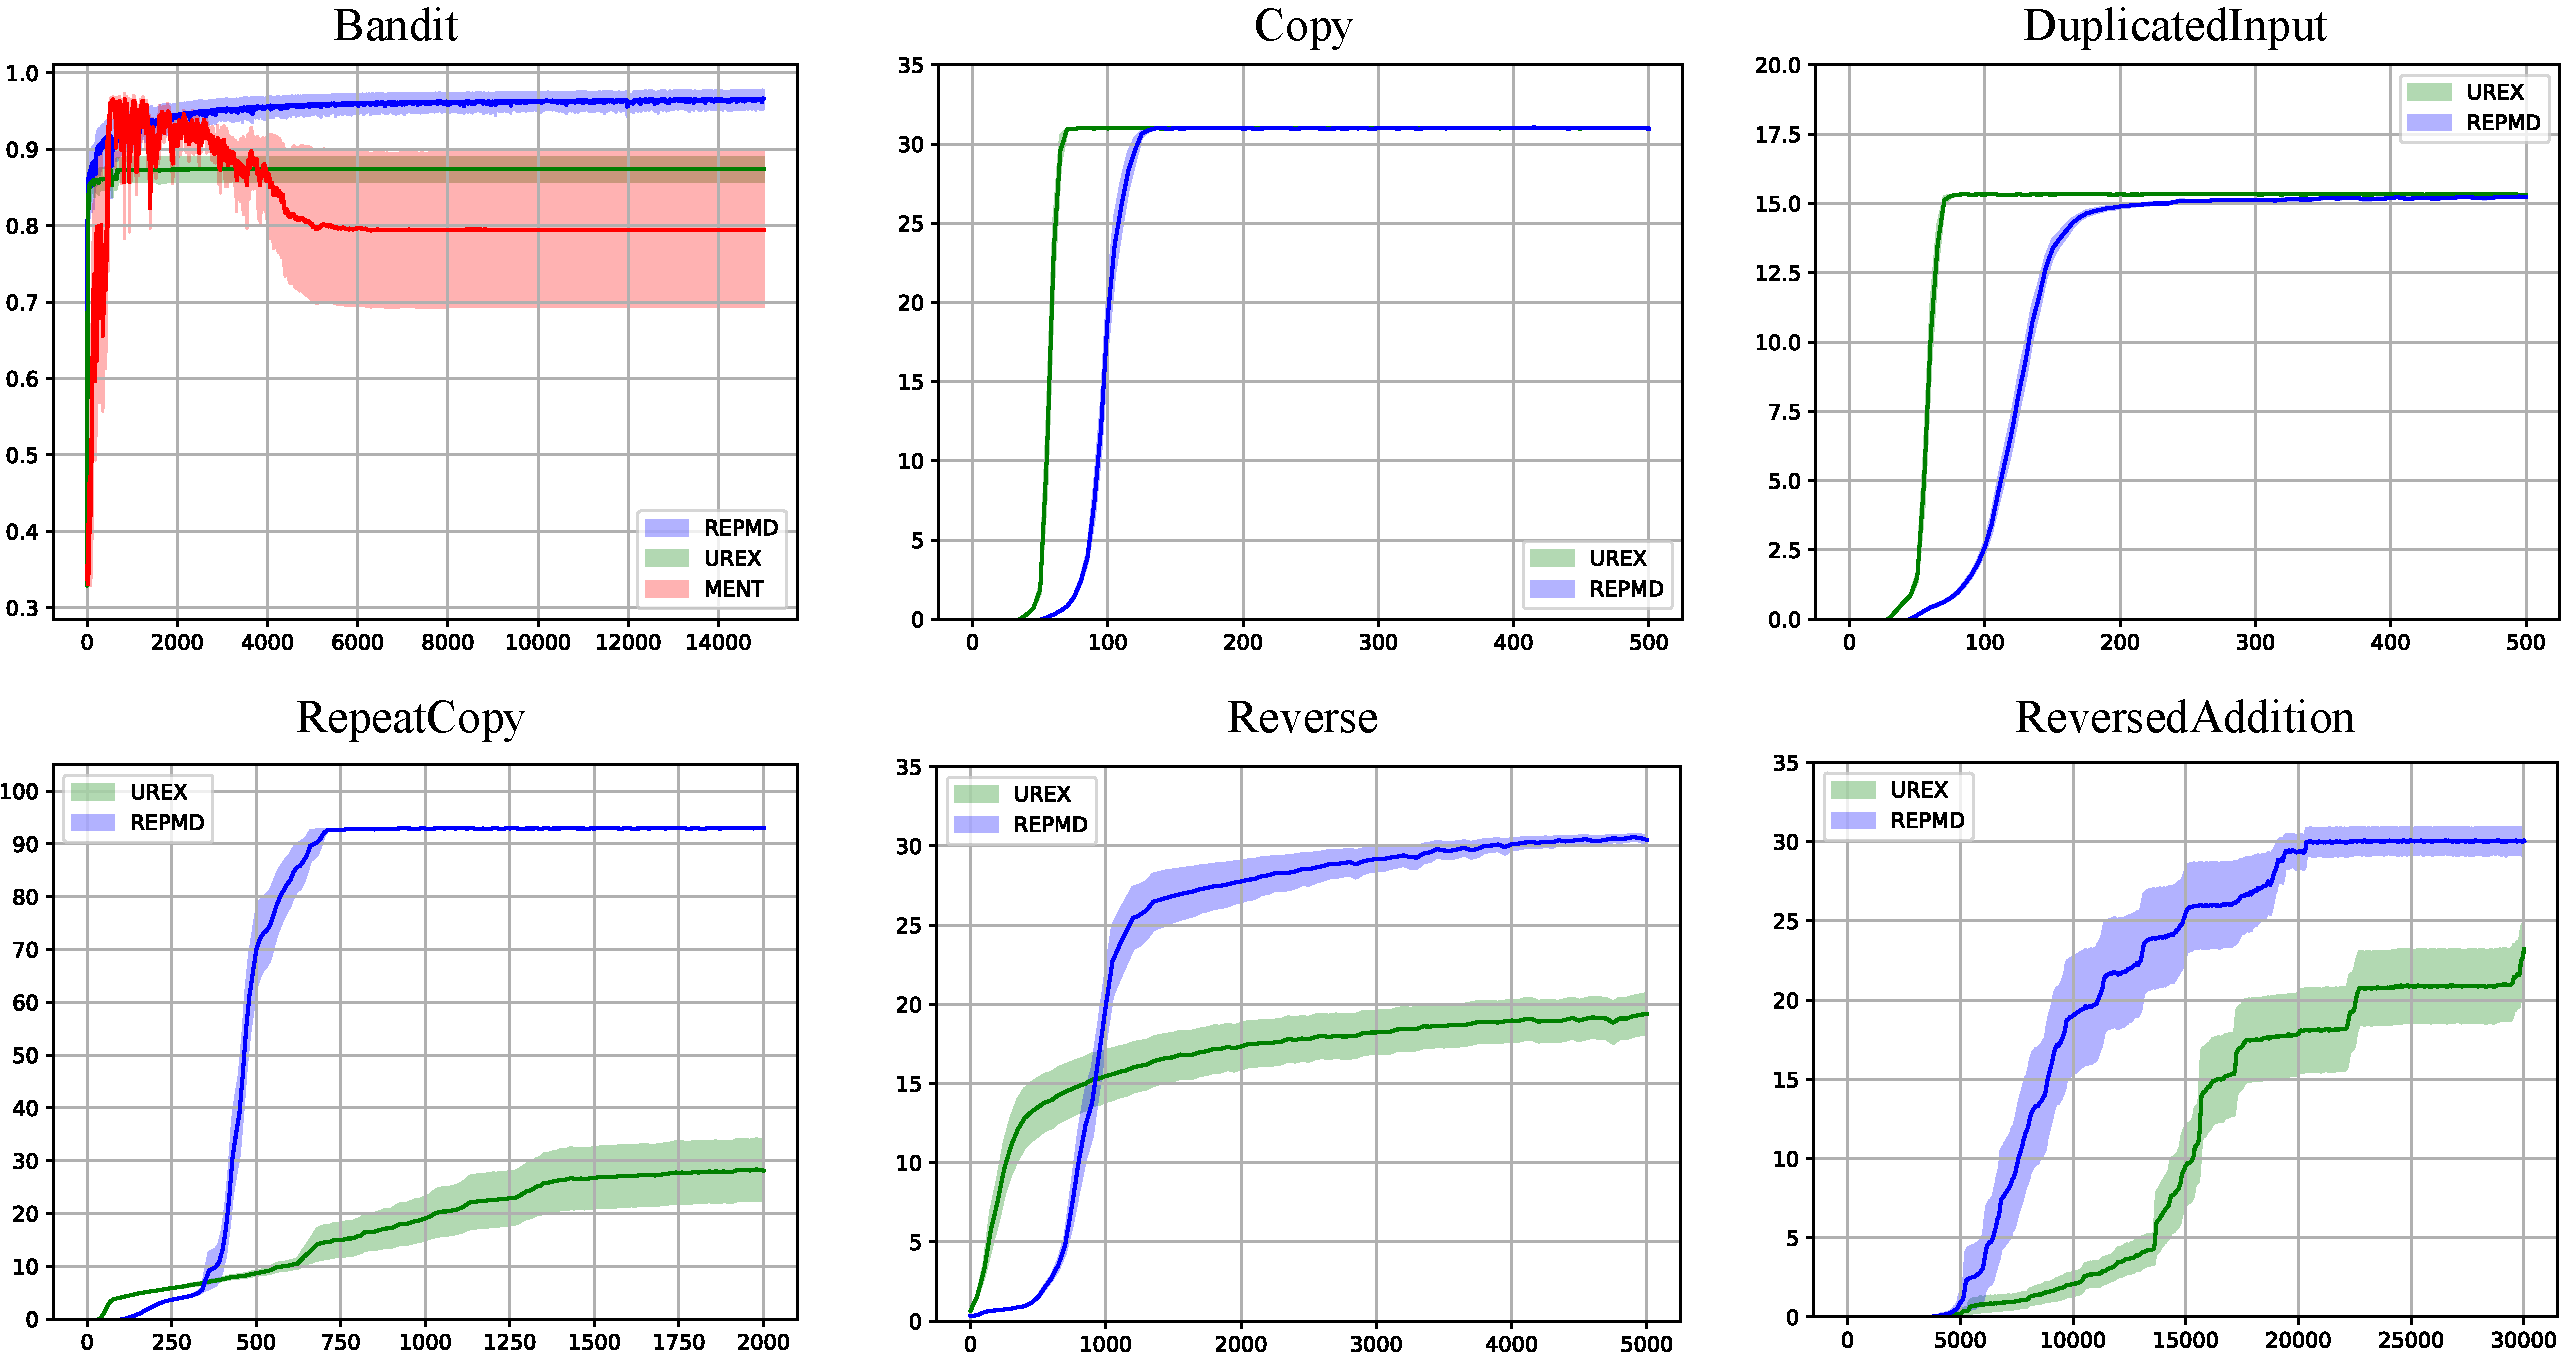
\includegraphics[width=0.8\linewidth]{./fig1.pdf}
\end{center}
\caption{
Results of MENT (red), UREX (green), and REPMD (blue) on synthetic bandit problem and algorithmic tasks. Plots show average reward with standard error during training. Synthetic bandit results averaged over 5 runs. Algorithmic task results averaged over 25 random training runs (5 runs $\times$ 5 random seeds for neural network initialization). X-axis is number of sampled trajectories. } 
\label{fig:results}
\end{figure*}

\subsection{Comparative Evaluation of REPMD}

For both synthetic bandit problem and algorithmic tasks, we compare REPMD against REINFORCE with entropy regularization (MENT) \citep{williams1992simple} and under-appreciated reward exploration (UREX) \citep{nachum2017improving}. Note that UREX is the state-of-the-art policy-based algorithm in algorithmic tasks. The results are reported in Figure (\ref{fig:results}). It is clear that REPMD substantially outperforms the competitors on all of these benchmark tasks. REPMD is able to consistently achieve the highest score and learn substantially faster than UREX. We also find the performance of UREX is very unstable. On the difficult tasks, including RepeatCopy, Reverse and ReversedAddition, UREX can only successfully find appropriate solutions a few times out of 5 runs for each random seed, which brings the overall scores down. This observation creates the gap between our presented results with the ones reported in the paper\footnote{The results reported in \citet{nachum2017improving} averages over 5 runs of random restart, while our results are averaged over 25 random training runs (5 runs $\times$ 5 random seed for neural network initialization). }. Note that the performance of REPMD is sill significantly better than UREX even compared with the results reported in \citet{nachum2017improving}. 

\subsubsection{Comparative Evaluation of PMAC}

We compare PMAC to deep deterministic policy gradient (DDPG) \citep{lillicrap2015continuous}, an efficient off-policy deep
RL methods, twin delayed deep deterministic policy gradient algorithm (TD3) \citep{fujimoto2018addressing}, a recent extension to DDPG by applying the double Q-learning trick to address over-estimation problem when function approximations are adopted, and Soft-Actor-Critic (SAC) \citep{haarnoja2018soft}, a recent state-of-the-art off-policy algorithm on a number of continuous control benchmarks. All these algorithms are implemented in rlkit \footnote{https://github.com/vitchyr/rlkit}. We do not include TRPO and PPO as our baselines in the experiments since their performance are dominated by SAC and TD3 as shown in \citep{haarnoja2018soft,fujimoto2018addressing}. 

\cref{fig:result_mujoco} presents the total mean return of evaluation rollouts during training of all algorithms. Results of each algorithm are averaged over five different instances with different random seeds. The solid curves corresponds to the mean and the shaded region to the standard errors over the five trials. For fair comparison with PMAC, we implement the double-Q but not the reparameterization trick (see equation (11)-(13) in \citep{haarnoja2018soft}) for SAC, which expains the discrepancy with the reported results in \citep{haarnoja2018soft}. We observe that without the reparameterization trick SAC cannot make any progress in the hardest problem Humanoid. To clarify this we also report the result of SAC with such trick on Humanoid using the author's GitHub implementation. The results show that PMAC matches or, in many cases, surpasses all other baseline algorithms in both final performance and sample efficiency across all tasks. In Humanoid, although PMAC is outperformed in the learning speed, its final performance is still comparable with SAC. Note that the reparameterization trick could also be applied in PMAC. We will include this in PMAC in the future work.

\begin{figure*}[t]
\begin{center}
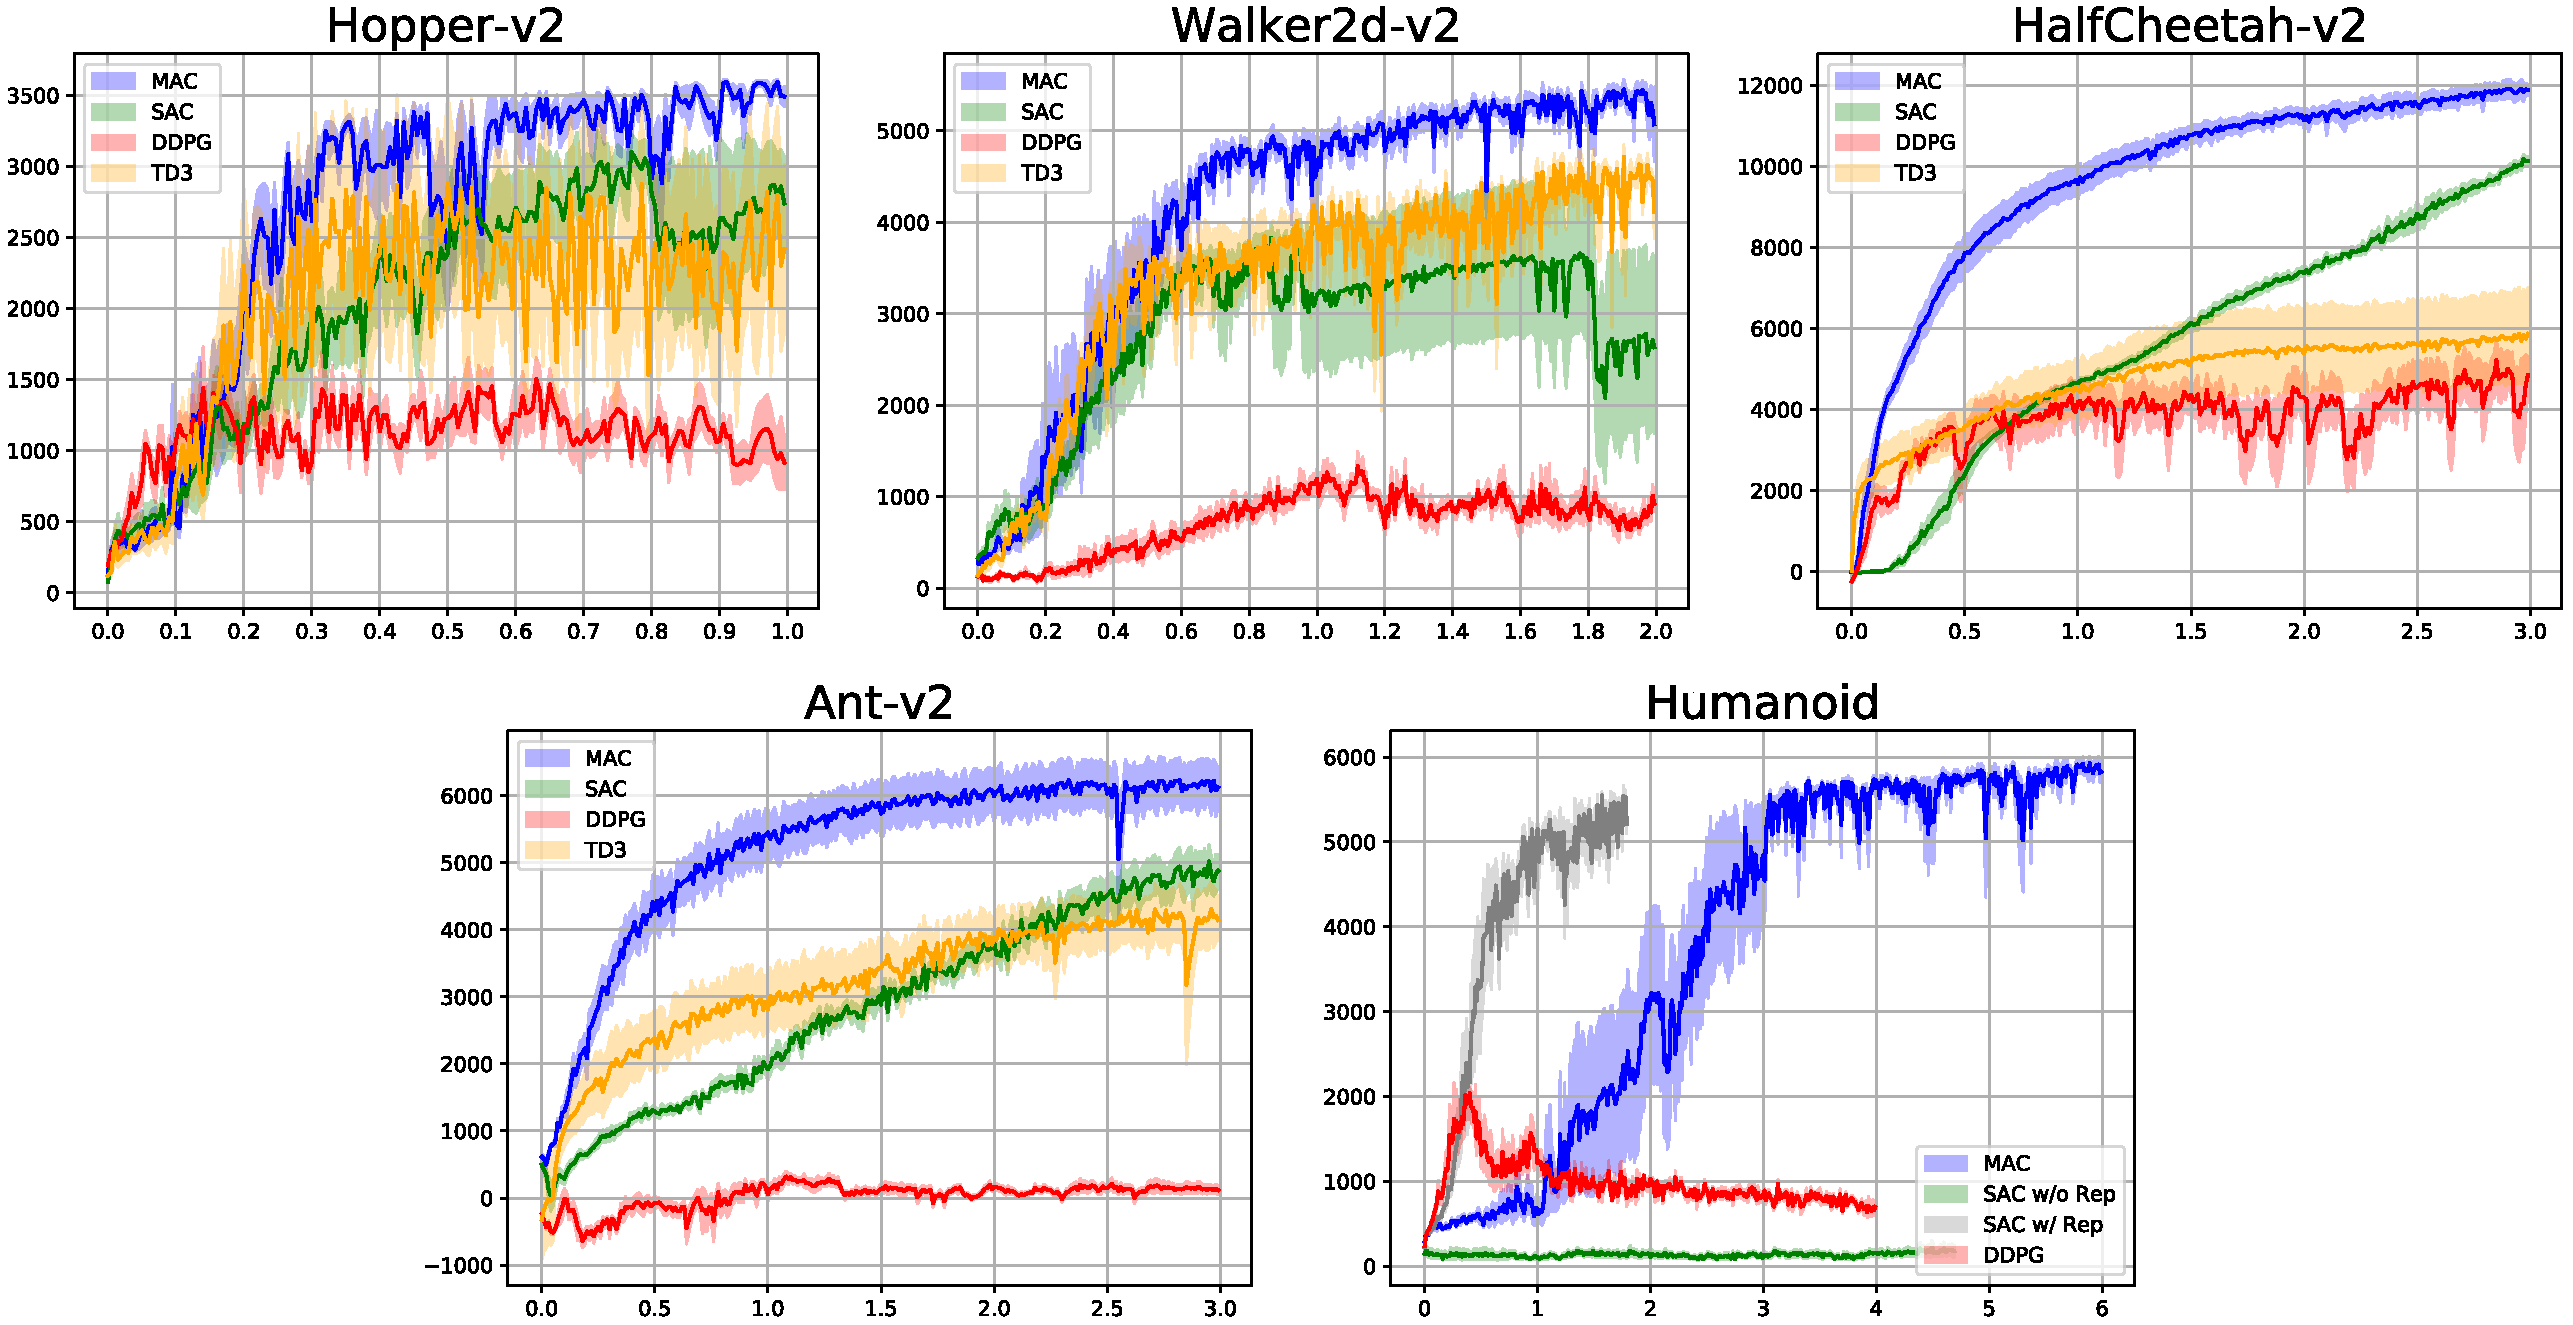
\includegraphics[width=0.85\linewidth]{./mujoco-results.pdf}
\end{center}
\caption{
Learning curves of DDPG (red), TD3 (yellow), SAC (green) and PMAC (blue) on mujoco tasks. Plots show mean reward with standard error during training, averaged over five different instances with different random seeds. X-axis is millions of environment steps. We observe that PMAC is consistently able to math and, in many cases, outperform all baseline algorithms across all tasks, both in terms of final performance and sample efficiency. }
\label{fig:result_mujoco } 
\end{figure*}


%\begin{wrapfigure}{R}{0.5\textwidth}
%\label{fig:ablation}
%  \begin{center}
%    \includegraphics[width=0.5\textwidth]{Copy.png}
%  \end{center}
%  \caption{Hello, Bye!}
%\end{wrapfigure}

\subsection{Ablation Study}
\label{subsec:ablationstudy}

The comparative evaluations provided in the previous sections suggest that our proposed algorithms based on the policy optimization method \ref{eq:repmd} outperform conventional RL methods on a number of challenging benchmarks. In this section, we further investigate how each novel component of \cref{eq:repmd} boosts the learning performance, by performing an ablation study on the most challenging algorithmic task ReversedAddition. 

%\piccaption[]{Ablation Study.\label{fig:ablation}}
%\parpic[r]{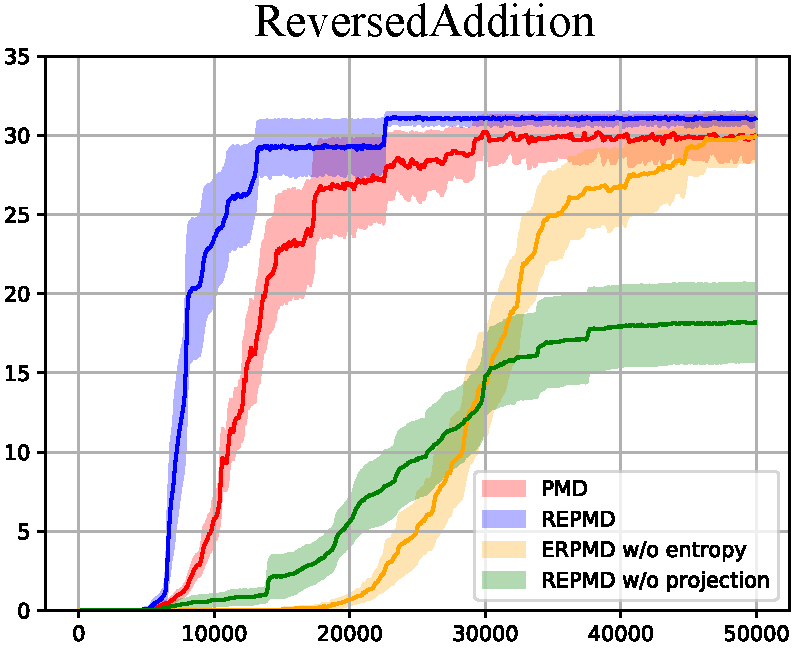
\includegraphics[width=0.35\linewidth]{ablation.pdf}}

\textbf{Importance of entropy regularizer.} The main difference between the function objective in \cref{eq:repmd} with the PMD objective \cref{eq:pmd} is to add another entropy regularizer. We demonstrate the importance of this choice by presenting the results of REPMD without the extra entropy regularizer, i.e. $\tau'=0$.

\textbf{Importance of KL divergence projection.} Another important difference between \cref{eq:repmd} with other RL methods is to use a project step to optimize policy, rather than direct SGD of the objective function. To show the importance of the project step, we test REPMD without projection, which only performs one step of gradient update at each iteration of training. 

\textbf{Importance of direction of KL divergence.} We choose PMD \ref{eq:pmd} as another baseline to prove the effectiveness of using the \emph{mean seeking} direction of KL divergence in the project step. Similar as in REPMD, we add a separate tempreture parameter $\tau'\geq 0$ to the original objective function in (\ref{eq:pmd}) to encourage exploration of the policy, which gives $\argmax_{\pi_\theta \in \Pi}{ \ep_{\rho \sim \pi_\theta}{  r(\rho)  - \tau \text{KL}(\pi_\theta \| \refPi) } + \tau'\cH(\pi_\theta) }$.

\begin{figure*}[t]
\begin{minipage}{0.5\linewidth}
\raggedleft
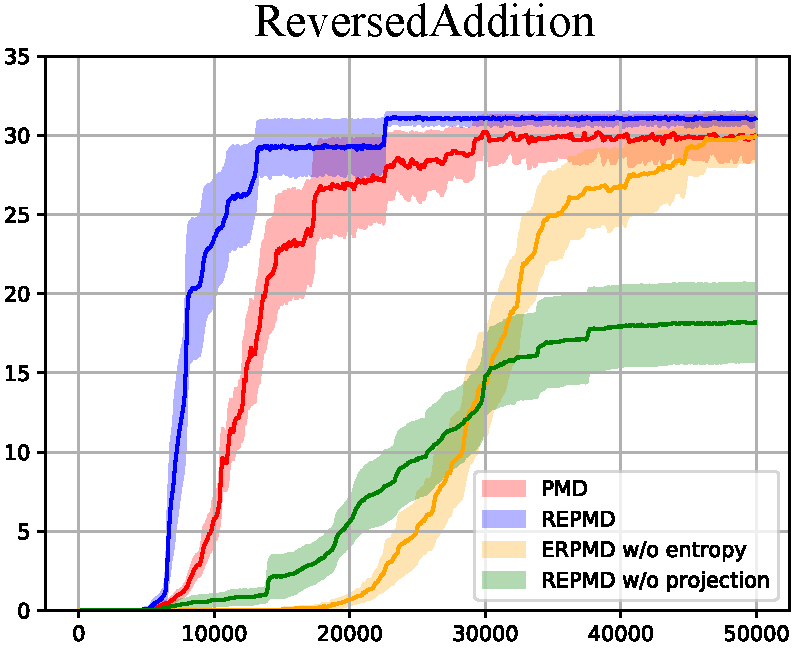
\includegraphics[width=1.6in]{./ablation.pdf}
\end{minipage}%
\begin{minipage}{0.5\linewidth}
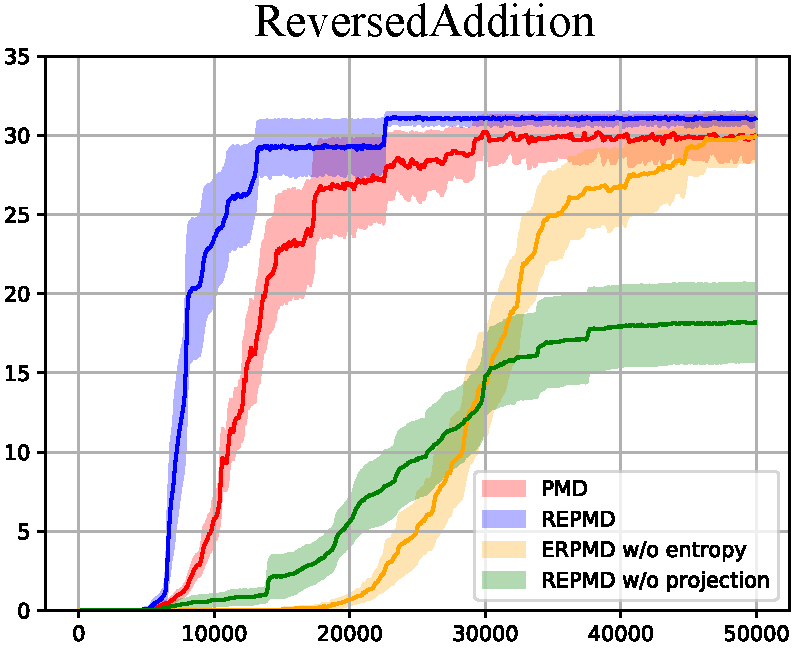
\includegraphics[width=1.6in]{./ablation.pdf}
%\caption{Error rate}
%\label{a}
\end{minipage}%

\caption{Ablation Study. ...}
\label{fig:result_mujoco}
\end{figure*}
